\ifdefined\maindoc\else
% typesetting this chapter as a standalone document
\def\doctitle{Muscle Wrapping and Via Points}
% starting definitions for both the main document and stand-alone chapters
\documentclass{book}

\def\mech{artisynth.core.mechmodels}
\def\mgeo{maspack.geometry}

% Add search paths for input files
\makeatletter
\def\input@path{{../}{../../}{../texinputs/}}
\makeatother

\usepackage{amsmath}
\usepackage{framed}
%%
%% Default settings for artisynth
%%
\NeedsTeXFormat{LaTeX2e}
%%\ProvidesPackage{artisynthDoc}[2012/04/05]

\usepackage[T1]{fontenc}
\usepackage[latin1]{inputenc}
\usepackage{listings}
\usepackage{makeidx}
\usepackage{latexml}
\usepackage{graphicx}
\usepackage{framed}
\usepackage{booktabs}
\usepackage{color}

\newcommand{\pubdate}{\today}
\newcommand{\setpubdate}[1]{\renewcommand{\pubdate}{#1}}
\newcommand{\code}[1]{{\tt #1}}

\iflatexml
\usepackage{hyperref}
\setlength\parindent{0pt} 
\else
%% then we are making a PDF, so include things that LaTeXML can't handle: 
%% docbook style, \RaggedRight
\usepackage{ifxetex}
\usepackage{xstring}
\usepackage{pslatex} % fixes fonts; in particular sets a better-fitting \tt font

\usepackage[most]{tcolorbox}
\definecolor{shadecolor}{rgb}{0.95,0.95,0.95}
\tcbset{
    frame code={}
    center title,
    left=0pt,
    right=0pt,
    top=0pt,
    bottom=0pt,
    colback=shadecolor,
    colframe=white,
    width=\dimexpr\textwidth\relax,
    enlarge left by=0mm,
    boxsep=0pt,
    arc=0pt,outer arc=0pt,
}%

\usepackage[A4]{artisynth_papersize}
%\usepackage[letter]{artisynth_papersize}
\usepackage[hyperlink]{asciidoc-dblatex} 

%\usepackage{verbatim}
\usepackage{ragged2e}
\setlength{\RaggedRightRightskip}{0pt plus 4em}
\RaggedRight
\renewcommand{\DBKpubdate}{\pubdate}
\renewcommand{\DBKreleaseinfo}{}
\fi

% set hypertext links to be dark blue:
\definecolor{darkblue}{rgb}{0,0,0.8}
\definecolor{sidebar}{rgb}{0.5,0.5,0.7}
\hypersetup{colorlinks=true,urlcolor=darkblue,linkcolor=darkblue,breaklinks=true}

%%%%%%%%%%%%%%%%%%%%%%%%%%%%%%%%%%%%%%%%%%%%%%%%%%%%%%%%%%%%%%%%%%%%%%%%%%%%%
%
% Define macros for handling javadoc class and method references
%
%%%%%%%%%%%%%%%%%%%%%%%%%%%%%%%%%%%%%%%%%%%%%%%%%%%%%%%%%%%%%%%%%%%%%%%%%%%%%
\makeatletter

% macro to enable line break if inside a PDF file
\def\pdfbreak{\iflatexml\else\\\fi}

% code inspired by http://stackoverflow.com/questions/2457780/latex-apply-an-operation-to-every-character-in-a-string
\def\removeargs #1{\doremoveargs#1$\wholeString\unskip}
\def\doremoveargs#1#2\wholeString{\if#1$%
\else\if#1({()}\else{#1}\taketherest#2\fi\fi}
\def\taketherest#1\fi
{\fi \doremoveargs#1\wholeString}

% Note: still doesn't work properly when called on macro output ...
% i.e., \dottoslash{\concatnames{model}{base}{foo}} fails 
\def\dottoslash #1{\dodottoslash#1$\wholeString\unskip}
\def\dodottoslash#1#2\wholeString{\if#1$%
\else\if#1.{/}\else{#1}\fi\dottaketherest#2\fi}
\def\dottaketherest#1\fi{\fi \dodottoslash#1\wholeString}

\def\hashtodot #1{\dohashtodot#1$\wholeString\unskip}
\def\dohashtodot#1#2\wholeString{\if#1$X%
\else\if#1\#{.}\else{#1}\fi\hashtaketherest#2\fi}
\def\hashtaketherest#1\fi{\fi \dohashtodot#1\wholeString}

%\dollartodot{#1} does the same thing as \StrSubstitute[0]{#1}{\$}{.}
% from the packahe xstring. We define \dollartodot instead because
% LaTeXML does not implement xstring.
%
% Note that for the substituion to work, we need \ifx instead of \if,
% since otherwise escaped characters won't work properly:
% if #1 = \$, then \if#1* seems to compare '\' and '$' (and output '*'),
% rather than comparing '$' to '*'
\def\dollartodot #1{\dodollartodot#1*\wholeString\unskip}
\def\dodollartodot#1#2\wholeString{\ifx#1*%
\else \ifx#1\${.}\else{#1}\fi\dollartaketherest#2\fi}
\def\dollartaketherest#1\fi{\fi \dodollartodot#1\wholeString}

% concatenates up to three class/method names together, adding '.' characters
% between them. The first and/or second argument may be empty, in which case
% the '.' is omitted. To check to see if these arguments are empty, we
% use a contruction '\if#1@@', which will return true iff #1 is empty
% (on the assumption that #1 will not contain a '@' character).
\def\concatnames
#1#2#3{\if#1@@\if#2@@#3\else #2.#3\fi\else\if#2@@#1.#3\else#1.#2.#3\fi\fi}

\newcommand{\javabase}{}
\newcommand{\setjavabase}[1]{\renewcommand{\javabase}{#1}}

\def\artisynthDocBase{@ARTISYNTHDOCBASE}

\iflatexml
\def\ifempty#1{\def\temp{#1}\ifx\temp\empty}%
\newcommand{\artisynthManual}[3][]{%
   \ifempty{#1}
      \href{@ARTISYNTHDOCBASE/#2/#2.html}{#3}%
    \else
      \href{@ARTISYNTHDOCBASE/#1/#2.html}{#3}%
    \fi
}
\else
\newcommand{\artisynthManual}[3][]{%
\href{https://www.artisynth.org/@ARTISYNTHDOCBASE/#2.pdf}{#3}}
\fi

%\href{@ARTISYNTHDOCBASE/#2/#2.html}{#3}}



\newcommand{\javaclassx}[2][]{%
% Includes code to prevent an extra '.' at the front if #1 is empty. It
% works like this: if '#1' is empty, then '#1.' expands to '.', and so 
% '\if#1..' will return true, in which case we just output '#2'.
\href{@JDOCBEGIN/\concatnames{\javabase}{#1}{#2}@JDOCEND}{#2}}
\newcommand{\javaclass}[2][]{%
\href{@JDOCBEGIN/\concatnames{}{#1}{#2}@JDOCEND}{\dollartodot{#2}}}
\newcommand{\javaclassAlt}[2]{%
\href{@JDOCBEGIN/\concatnames{}{}{#1}@JDOCEND}{#2}}

\newcommand{\javamethodArgsx}[2][]{%
\href{@JDOCBEGIN/\concatnames{\javabase}{#1}{#2}@JDOCEND}{#2}}
\newcommand{\javamethodArgs}[2][]{%
\href{@JDOCBEGIN/\concatnames{}{#1}{#2}@JDOCEND}{#2}}
\newcommand{\javamethodAlt}[2]{%
\href{@JDOCBEGIN/\concatnames{}{}{#1}@JDOCEND}{#2}}
\newcommand{\javamethodAltx}[2]{%
\href{@JDOCBEGIN/\concatnames{\javabase}{}{#1}@JDOCEND}{#2}}

\newcommand{\javamethodNoArgsx}[2][]{%
\href{@JDOCBEGIN/\concatnames{\javabase}{#1}{#2}@JDOCEND}{\removeargs{#2}}}
\newcommand{\javamethodNoArgs}[2][]{%
\href{@JDOCBEGIN/\concatnames{}{#1}{#2}@JDOCEND}{\removeargs{#2}}}

\newcommand{\javamethod}{\@ifstar\javamethodNoArgs\javamethodArgs}
\newcommand{\javamethodx}{\@ifstar\javamethodNoArgsx\javamethodArgsx}

%%%%%%%%%%%%%%%%%%%%%%%%%%%%%%%%%%%%%%%%%%%%%%%%%%%%%%%%%%%%%%%%%%%%%%%%%%%%%
%
% Define macros for sidebars
%
%%%%%%%%%%%%%%%%%%%%%%%%%%%%%%%%%%%%%%%%%%%%%%%%%%%%%%%%%%%%%%%%%%%%%%%%%%%%%

\iflatexml
\newenvironment{sideblock}{\begin{quote}}{\end{quote}}
\else
\usepackage[strict]{changepage}
\definecolor{sidebarshade}{rgb}{1.0,0.97,0.8}
\newenvironment{sideblock}{%
    \def\FrameCommand{%
    \hspace{1pt}%
    {\color{sidebar}\vrule width 2pt}%
    %{\vrule width 2pt}%
    {\color{sidebarshade}\vrule width 4pt}%
    \colorbox{sidebarshade}%
  }%
  \MakeFramed{\advance\hsize-\width\FrameRestore}%
  \noindent\hspace{-4.55pt}% disable indenting first paragraph
  \begin{adjustwidth}{}{7pt}%
  %\vspace{2pt}\vspace{2pt}%
}
{%
  \vspace{2pt}\end{adjustwidth}\endMakeFramed%
}
\fi

\iflatexml
\newenvironment{shadedregion}{%
  \definecolor{shadecolor}{rgb}{0.96,0.96,0.98}%
  \begin{shaded*}%
% Put text inside a quote to create a surrounding blockquote that
% will properly accept the color and padding attributes
  \begin{quote}%
}
{%
  \end{quote}%
  \end{shaded*}%
}
\else
\newenvironment{shadedregion}{%
  \definecolor{shadecolor}{rgb}{0.96,0.96,0.98}%
  \begin{shaded*}%
}
{%
  \end{shaded*}%
}
\fi

% Wanted to create a 'listing' environment because lstlisting is
% tedious to type and because under latexml it may need
% some massaging to get it to work properly. But hard to do
% because of the verbatim nature of listing
%\iflatexml
%\newenvironment{listing}{\begin{lstlisting}}{\end{lstlisting}}%
%\else
%\newenvironment{listing}{\begin{lstlisting}}{\end{lstlisting}}%
%\fi

\iflatexml\else
% fancyhdr was complaining that it wanted a 36pt header height ...
\setlength{\headheight}{36pt}
\fi

% macro for backslash character
\newcommand\BKS{\textbackslash}

% macro for double hyphen (to prevent conversion of -- into -)
\newcommand\DHY{-{}-}

% Convenience stuff
\newcommand{\ifLaTeXMLelse}[2]{%
  \iflatexml %
  #1 %
  \else %
  #2 %
  \fi %
}

\newcommand{\ifLaTeXML}[1]{ %
  \iflatexml %
  #1 %
  \fi %
}

% new methodtable environment for documenting methods

% base width of the method table
\newlength{\methodtablewidth}
\iflatexml
\setlength{\methodtablewidth}{1.4\textwidth}
\else
\setlength{\methodtablewidth}{0.94\textwidth}
\fi
% horizontal space added at end of call to \methodentry
\newlength{\methodskip}
\setlength{\methodskip}{0pt}
% lengths set inside methodtable environment:
\newlength{\methodsiglength} % length of the method signature
\newlength{\methodcomlength} % length of the method comment
\setlength{\methodsiglength}{0.5\methodtablewidth}
\setlength{\methodcomlength}{0.5\methodtablewidth}

% command to add a method to a method table:
% arg #1: package and signature for finding URL
% arg #2: anchor text
% arg #3: comment describing the method
\newcommand{\methodentry}[3]{%
\javamethodAlt{#1}{\parbox[t]{\methodsiglength}{#2}}&
{\parbox[t]{\methodcomlength}{#3}}\\%
\noalign{\vspace{\methodskip}}}

% methodtable environment takes two arguments, both scale factors for
% methodtablewidth:
% arg #1: width of the method signature column
% arg #2: width of the method comment column
\newenvironment{methodtable}[3][0pt]{%
\begingroup
\setlength{\topskip}{0pt}
\setlength{\methodskip}{#1}
\setlength{\methodsiglength}{#2\methodtablewidth}%
\setlength{\methodcomlength}{#3\methodtablewidth}%
\iflatexml
\begin{snugshade}
\else
\begin{tcolorbox}
\fi
\renewcommand{\arraystretch}{1}
\begin{tabular}{ll}}{%
\end{tabular}
\renewcommand{\arraystretch}{1}
\iflatexml
\end{snugshade}
\else
\end{tcolorbox}
\fi
\endgroup}

% commands for added top, mid and bottom lines in the table.
% uses booktabs for PDF, regular hline for HTML
\newcommand{\topline}{\iflatexml\hline\else\toprule\fi}
\newcommand{\midline}{\iflatexml\hline\else\midrule\fi}
\newcommand{\botline}{\iflatexml\hline\else\bottomrule\fi}
\newcommand{\blankline}{%
\multicolumn{2}{l}{\iflatexml{@SPACE}\else\phantom{M}\fi}\\}%
% add vertical space within a two colum method environment
\newcommand{\methodspace}[1]{%
\iflatexml
\multicolumn{2}{l}{@VERTSPACE[#1]}\\
\else
\noalign{\vspace{#1}}%
\fi}%
% break a line and add an indentation of 1em
\newcommand{\brh}{\\\phantom{M}}

\makeatother

\def\matl{\left(\begin{matrix}}
\def\matr{\end{matrix}\right)}

\def\Bthe{\boldsymbol\theta}
\def\Btau{\boldsymbol\tau}
\def\Bom{\boldsymbol\omega}
\def\Bdel{\boldsymbol\delta}
\def\Blam{\boldsymbol\lambda}
\def\Bphi{\boldsymbol\phi}
\def\Bxi{\boldsymbol\xi}
\def\Bgam{\boldsymbol\gamma}
\def\Bsig{\boldsymbol\sigma}
\def\Bnu{\boldsymbol\nu}
\def\Bmu{\boldsymbol\mu}

\def\A{{\bf A}}
\def\B{{\bf B}}
\def\C{{\bf C}}
\def\D{{\bf D}}
\def\F{{\bf F}}
\def\G{{\bf G}}
\def\H{{\bf H}}
\def\I{{\bf I}}
\def\J{{\bf J}}
\def\K{{\bf K}}
\def\Jc{{\bf J}_c}
\def\L{{\bf L}}
\def\M{{\bf M}}
\def\N{{\bf N}}
\def\O{{\bf O}}
\def\P{{\bf P}}
\def\Q{{\bf Q}}
\def\R{{\bf R}}
\def\T{{\bf T}}
\def\U{{\bf U}}
\def\W{{\bf W}}
\def\X{{\bf X}}
\def\Minv{{\bf M}^{-1}}

\def\a{{\bf a}}
\def\b{{\bf b}}
\def\c{{\bf c}}
\def\d{{\bf d}}
\def\e{{\bf e}}
\def\f{{\bf f}}
\def\g{{\bf g}}
\def\k{{\bf k}}
\def\l{{\bf l}}
\def\m{{\bf m}}
\def\n{{\bf n}}
\def\p{{\bf p}}
\def\q{{\bf q}}
\def\r{{\bf r}}
\def\u{{\bf u}}
\def\v{{\bf v}}
\def\w{{\bf w}}
\def\x{{\bf x}}
\def\y{{\bf y}}
\def\z{{\bf z}}

\def\ma{{\bf m}_\alpha}
\def\mb{{\bf m}_\beta}
\def\va{{\bf v}_\alpha}
\def\vb{{\bf v}_\beta}
\def\vp{{\bf v}_\rho}
\def\vk{{\bf v}_k}
\def\ua{{\bf u}_\alpha}
\def\ub{{\bf u}_\beta}
\def\uk{{\bf u}_k}
\def\uj{{\bf u}_j}
\def\mar{{\bf m}_{\alpha r}}
\def\mbr{{\bf m}_{\beta r}}

\def\Maa{{\bf M}_{\alpha\alpha}}
\def\Mab{{\bf M}_{\alpha\beta}}
\def\Mba{{\bf M}_{\beta\alpha}}
\def\Mbb{{\bf M}_{\beta\beta}}
\def\hatMaa{\hat{\bf M}_{\alpha\alpha}}
\def\hatMab{\hat{\bf M}_{\alpha\beta}}
\def\hatMba{\hat{\bf M}_{\beta\alpha}}
\def\hatMbb{\hat{\bf M}_{\beta\beta}}
\def\Mbp{{\bf M}_{\beta\rho}}
\def\Map{{\bf M}_{\alpha\rho}}
\def\Mpa{{\bf M}_{\rho\alpha}}
\def\Mpb{{\bf M}_{\rho\beta}}
\def\Mpp{{\bf M}_{\rho\rho}}
\def\Mbk{{\bf M}_{\beta k}}
\def\Mak{{\bf M}_{\alpha k}}
\def\Mka{{\bf M}_{k\alpha}}
\def\Mkb{{\bf M}_{k\beta}}
\def\Mkk{{\bf M}_{kk}}

\def\Ga{{\bf G}_{\alpha}}
\def\Gp{{\bf G}_{\rho}}
\def\Gaa{{\bf G}_{\alpha\alpha}}
\def\Gab{{\bf G}_{\alpha\beta}}
\def\Gba{{\bf G}_{\beta\alpha}}
\def\Gbb{{\bf G}_{\beta\beta}}
\def\Gap{{\bf G}_{\alpha\rho}}
\def\Gpa{{\bf G}_{\rho\alpha}}
\def\Gbp{{\bf G}_{\beta\rho}}
\def\Gak{{\bf G}_{\alpha k}}
\def\Gka{{\bf G}_{k\alpha}}
\def\Gja{{\bf G}_{j\alpha}}
\def\Gkb{{\bf G}_{k\beta}}
\def\Gbk{{\bf G}_{\beta k}}

\def\lama{\Blam_{\alpha}}
\def\lamb{\Blam_{\beta}}
\def\lamp{\Blam_{\rho}}
\def\lamk{\Blam_{k}}
\def\lams{\Blam_{\sigma}}

\def\ba{{\bf b}_{\alpha}}
\def\bb{{\bf b}_{\beta}}
\def\fp{{\bf f}_{\rho}}
\def\fa{{\bf f}_{\alpha}}
\def\qa{{\bf q}_{\alpha}}
\def\qb{{\bf q}_{\beta}}
\def\za{{\bf z}_{\alpha}}
\def\zb{{\bf z}_{\beta}}
\def\wa{{\bf w}_{\alpha}}
\def\wb{{\bf w}_{\beta}}

\def\Na{\bar{\bf N}_{\alpha}}
\def\Nb{\bar{\bf N}_{\beta}}

\def\Up{{\bf U}_p}
\def\Un{{\bf U}_n}

\def\dFdl{\frac{\partial F}{\partial l}}
\def\dFddl{\frac{\partial F}{\partial \dot l}}

\def\Sr{s_\theta}
\def\Cr{c_\theta}
\def\Sp{s_\phi}
\def\Cp{c_\phi}
\def\Sy{s_\psi}
\def\Cy{c_\psi}
\def\Sa{s_{\alpha}}
\def\Ca{c_{\alpha}}
\def\Vp{v_{\phi}}


\iflatexml
\else
\usepackage{biblatex}
\addbibresource{references.bib}
\fi

\setcounter{tocdepth}{5}
\setcounter{secnumdepth}{3}

\title{\doctitle}
\ifdefined\maindoc
\author{John Lloyd and Antonio S\'anchez}
\setpubdate{Last update: March, 2022}

\iflatexml
\date{}
\fi
\fi

% graphics paths
\graphicspath{{./}{images/}}

% Listings settings
\definecolor{myblue}{rgb}{0,0,0.6}
\definecolor{mygreen}{rgb}{0,0.6,0}
\definecolor{mygray}{rgb}{0.5,0.5,0.5}
\definecolor{mylightgray}{rgb}{0.95,0.95,0.95}
\definecolor{mymauve}{rgb}{0.58,0,0.82}
\definecolor{myblack}{rgb}{0,0,0}
\lstset{
   language=Java,                   % text highlighting for Java
   breakatwhitespace=false,         % automatic breaks only at whitespace
   breaklines=true,                 % automatic line breaking
   commentstyle=\color{mygreen},    % comment style
   keepspaces=true,                 % keeps spaces in text
   keywordstyle=\color{myblue},     % keyword style
   numbers=none,                    % line-numbers; values: (none, left, right)
   numbersep=5pt,                   % how far the line-numbers are from code
   numberstyle=\tiny\color{mygray}, % line-numbers style
   showspaces=false,                % show spaces everywhere
   showstringspaces=false,          % underline spaces within strings
   showtabs=false,                  % show tabs
   stepnumber=1,                    % the step between two line-numbers
   stringstyle=\color{mymauve},     % string literal style
   tabsize=3,                       % sets default tabsize to 3 spaces
   backgroundcolor=\color{mylightgray}, % background color
   frame=single, 					% adds a frame around the code
   rulesepcolor=\color{mygray},
   rulecolor=\color{myblack},
   framerule=0pt,
   xleftmargin=2.2ex,               % numbers inside box
   framexleftmargin=2.2ex,			% indentation of frame
}

\begin{document}

\frontmatter

%\layout
\maketitle

\iflatexml{\large\pubdate}\fi

\tableofcontents

\mainmatter
\fi

\chapter{Muscle Wrapping and Via Points}
\label{multipointSpringIntro:sec}

ArtiSynth provides support for multipoint springs and muscles, which
are similar to axial springs and muscles (Sections
\ref{AxialSprings:sec} and \ref{PointToPointMuscles:sec}), except that
they can contain multiple via points and also wrap around obstacles.
This allows the associated force directions to vary in response to
obstacles and constraints in the model, which is particularly
important in biomechanical models where point-to-point muscles need to
wrap around anatomical structures such as bones.  A schematic
illustration is shown in Figure \ref{multiPointSpring:fig}, where a
single spring connects points $\p_0$ and $\p_2$, while passing through
a single via point $\p_1$ and wrapping around obstacles $W_1$ and
$W_2$. Figure \ref{multiSpringExamples:fig} shows two examples
involving a rigid body with fixed via points and a spring wrapping
around three rigid bodies.

\begin{figure}[ht]
\begin{center}
 \includegraphics[width=4in]{images/multiPointSpring}
\end{center}
\caption{Schematic illustration of a multipoint spring passing through
a via point $\p_1$ and wrapping around two obstacles $W_1$ and
$W_2$. The points $A_1$, $B_1$ and $A_2$, $B_2$ denote the first and
last locations where $W_1$ and $W_2$ make contact with the spring.}
\label{multiPointSpring:fig}
\end{figure}

\begin{figure}[ht]
\begin{center}
  \begin{tabular}{cc}
    \iflatexml
       \includegraphics[width=3in]{images/multiSpringDemo}&
       \includegraphics[width=3in]{images/multiBodyWrap2}
    \else
       \includegraphics[width=2.5in]{images/multiSpringDemo}&
       \includegraphics[width=2.5in]{images/multiBodyWrap2}
    \fi
  \end{tabular}
\end{center}
\caption{Left: A multipoint spring with two via points rigidly fixed
to a box-shaped rigid body. Right: A multipoint spring wrapped around
three obstacles.}
\label{multiSpringExamples:fig}
\end{figure}

As with axial springs and muscles, multipoint springs and muscles must
have two points to denote their beginning and end. In between, they can
have any number of {\it via} points, which are fixed locations which
the spring must pass through in the specified order. Any ArtiSynth
\javaclass[\mech]{Point} object may be specified
as a via point, including particles and markers. The purpose of the
via point is generally to direct the spring along some particular
path. In particular, the path directions before and after a via point
will generally be different, and forces acting on the via point will
be determined by the tension in the spring (or muscle) acting along
these two different directions.

\begin{figure}[ht]
\begin{center}
 \includegraphics[width=2.5in]{images/multiPointViaPoint}
\end{center}
\caption{A multipoint spring with a single via point $\p_1$, showing
the unit direction vectors $\u_A$ and $\u_B$ immediately before and
after.}
\label{multiPointViaPoint:fig}
\end{figure}

\begin{sideblock}
Conceptually, the spring or muscle ``slides'' through its via points,
which act analogously to virtual three dimensional pulleys. In
particular, the proportional distance between via points does {\it not}
remain fixed.
\end{sideblock}

The tension $f$ within the spring or muscle is computed from its
material, using the relation $f(l,\dot l, a)$ described in Sections
\ref{AxialSprings:sec} and \ref{sec:mechii:musclematerials},
where $l$ now denotes the {\it entire} length of the spring
as it passes through the via points and wraps around obstacles. The
total force $\f$ acting on each via point is then given by
%
\begin{equation*}
\f = f \cdot (\u_B - \u_A)
\end{equation*}
%
where $\u_B$ and $\u_A$ are unit vectors giving the spring's direction
immediately after and before the via point
(Figure \ref{multiPointViaPoint:fig}).

Multipoint springs can also be made to wrap around one or more {\it
wrappable} objects. Unlike via points, wrappable objects can occur in
any order along the spring and wrapping only occurs when the spring
and the object actually collide. Any ArtiSynth object that implements
\javaclass[\mech]{Wrappable} can be used as a wrapping object
(currently, only \javaclass[\mech]{RigidBody} objects
implement {\tt Wrappable}).
The forces acting on a wrappable are those
generated by the forces $\f_A$ and $\f_B$ acting on the points
A and B where the spring makes and leaves contact with the
it (Figure \ref{multiPointObstacle:fig}). These forces
are given by
%
\begin{equation*}
\f_A = - f \u_A, \quad \f_B = f \u_B,
\end{equation*}
%
where $\u_B$ are $\u_A$ are unit vectors giving the spring's direction
immediately before A and after B. Points A and B are collectively
known as the A/B points.

\begin{figure}[ht]
\begin{center}
 \includegraphics[width=2.5in]{images/multiPointObstacle}
\end{center}
\caption{A multipoint spring wrapping around a single obstacle $W$,
with initial and final contact at points A and B, 
and associated unit direction vectors $\u_A$ and $\u_B$.}
\label{multiPointObstacle:fig}
\end{figure}

\section{Via Points}
\label{ViaPoints:sec}

Multipoint springs and muscles are implemented by the classes
\javaclass[\mech]{MultiPointSpring} and
\javaclass[\mech]{MultiPointMuscle}, respectively.
The relationship between {MultiPointSpring} and 
{MultiPointMuscle} is the same as that between
\javaclass[\mech]{AxialSpring} and \javaclass[\mech]{Muscle}:
The latter is a subclass of the former, and allows
the creation of active tension forces in response to
its {\sf excitation} property.

An application allocates one of these components, sets the appropriate
material properties for the tension forces, and then adds points and
wrappable objects as desired.

Points can be added, queried, and removed using the methods
%
\begin{lstlisting}[]
   void addPoint (Point pnt)
   Point getPoint (int idx)
   int numPoints()
   boolean removePoint (Point pnt)
\end{lstlisting}
%
As with \javaclass[\mech]{AxialSpring}, there must
be at least two points anchoring the beginning and end of the
spring. Any additional points will be {\it via points}.

\begin{figure}[ht]
\begin{center}
  \begin{tabular}{cc}
    \iflatexml
       \includegraphics[width=3in]{images/cylinderWrapping}&
       \includegraphics[width=3in]{images/cylinderWrappingKnots}
    \else
       \includegraphics[width=2.5in]{images/cylinderWrapping}&
       \includegraphics[width=2.5in]{images/cylinderWrappingKnots}
    \fi
  \end{tabular}
\end{center}
\caption{A multipoint spring with two segments, separated by a blue
via point (top), with the rightmost segment set to be wrappable so
that it can wrap around a cylinder. The right image shows the
wrappable segment's knots.}
\label{cylinderWrappingKnots:fig}
\end{figure}

The section of a multipoint spring between any two adjacent points is
known as a {\it segment}. By default, each segment forms a straight
line between the two points and does {\it not} interact with any
wrappable obstacles. To interact with wrappables, a segment needs to
be declared {\it wrappable}, as described in
Section \ref{ObstacleWrapping:sec}.

Spring construction is illustrated by the following code fragment:
%
\begin{lstlisting}[]
   MultiPoint spring = new MultiPointSpring();
   spring.setMaterial (new LinearAxialMaterial (stiffness, damping));
   spring.addPoint (p0); // start point
   spring.addPoint (p1); // via point
   spring.addPoint (p2); // via point
   spring.addPoint (p3); // stop point
\end{lstlisting}
%
This creates a new {\tt MultiPointSpring} and sets its material to a
simple linear material with a specified stiffness and damping.  Four points
{\tt p0}, {\tt p1}, {\tt p2}, {\tt p3} are then added, forming a start
point, two via points, and a stop point.

\subsection{Example: a muscle with via points}
\label{ViaPointMuscle:sec}

\begin{figure}[t]
\begin{center}
\iflatexml
 \includegraphics[]{images/ViaPointMuscle}
\else
 \includegraphics[width=3.75in]{images/ViaPointMuscle}
\fi
\end{center}
\caption{ViaPointMuscle model loaded into ArtiSynth.}
\label{ViaPointMuscle:fig}
\end{figure}

A simple example of a muscle containing via points is given by 
{\tt artisynth.demos.tutorial.ViaPointMuscle}.  It consists
of a MultiPointMuscle passing through two via points attached to a
block. The code is given below:
\lstset{numbers=left}
\lstinputlisting{../../src/artisynth/demos/tutorial/ViaPointMuscle.java}
\lstset{numbers=none}

Lines 21-30 of the {\tt build()} method create a {\tt MechModel} and
add a simple rigid body block to it. Two non-dynamic points ({\tt p0}
and {\tt p1}) are then created to act as muscle end points
(lines 33-38), along with two markers ({\tt via0} and {\tt via1})
which are attached to the block to act as via points
(lines 41-44). The muscle itself is created by lines 42-53, with the
end points and via points being added in order from start to end.
The muscle material is a 
\javaclass[artisynth.core.materials]{SimpleAxialMuscle},
which computes tension according to the simple linear formula 
(\ref{SimpleAxialMuscle:eqn}) described in Section 
\ref{sec:mechii:musclematerials}. Lines 56-57 set render
properties for the model, and line 59 creates a control panel
(Section \ref{ControlPanels:sec}) that allows the muscle {\sf
excitation} property to be interactively controlled.

To run this example in ArtiSynth, select {\sf All demos > tutorial >
ViaPointMuscle} from the {\sf Models} menu. The model should load and
initially appear as in Figure \ref{ViaPointMuscle:fig}.  Running the
model will cause the block to fall and swing about under gravity,
while changing the muscle's {\sf excitation} in the control panel will
vary its tension.

\section{Obstacle Wrapping}
\label{ObstacleWrapping:sec}

As mentioned in Section \ref{ViaPoints:sec}, segments between pairs of
via points can be declared {\it wrappable}, allowing them to interact
with wrappable obstacles. This can be done as via points are added
to the spring, using the methods
%
\begin{lstlisting}[]
   void setSegmentWrappable (int numKnots)
   void setSegmentWrappable (int numKnots, Point3d[] initialPoints)
\end{lstlisting}
%
These make {\it wrappable} the next segment to be created (i.e., the segment
between the most recently added point and the next point to be added),
with {\tt numKnots} specifying the number of {\it knots} that should
be used to implement the wrapping. Knots are points that divide the
wrappable segment into a piecewise linear curve, and are used to
check for collisions with the wrapping surfaces
(Figure \ref{cylinderWrappingKnots:fig}).  The argument {\tt
initialPoints} used by the second method is an optional argument
which, if non-null, can be used to specify intermediate guide points
to give the segment an initial path around around any obstacles (for
more details, see Section \ref{wrappingInit:sec}).

Each wrappable segment will be capable of colliding with any of the
wrappable obstacles that are known to the spring.  Wrappables can be
added, queried and removed using the following methods:
%
\begin{lstlisting}[]
   void addWrappable (Wrappable wrappable)
   Wrappable getWrappable (int idx)
   int numWrappables()
   boolean removeWrappable (Wrappable wrappable)
\end{lstlisting}
%
Unlike points, however, there is no implied ordering and wrappables
can be added in any order and at any time during the spring's
construction.

Wrappable spring construction is illustrated by the following code
fragment:
%
\begin{lstlisting}[]
   MultiPoint spring = new MultiPointSpring();
   spring.setMaterial (new LinearAxialMaterial (stiffness, damping));
   spring.addPoint (p0); // start point
   spring.setSegmentWrappable (50);  // wrappable segment
   spring.addPoint (p1); // via point
   spring.addPoint (p2); // end point
   spring.addWrappable (wrappable1);
   spring.addWrappable (wrappable2);
   spring.updateWrapSegments(); // ``shrink wrap'' spring to the obstacles
\end{lstlisting}
%
This creates a new {\tt MultiPointSpring} with a linear material and
three points {\tt p0}, {\tt p1}, and {\tt p2}, forming a start point,
via point, and stop point.  The segment between {\tt p0} and {\tt p1}
is set to be wrappable with 50 knot points. Two wrappable obstacles
are added next, each of which will interact with the {\tt p0}-{\tt p1}
segment, but {\it not} with the non-wrappable {\tt p1}-{\tt p2}
segment. Finally, {\tt updateWrapSegments()} is called to do an
initial solve for the wrapping segments, so that they will be ``pulled
tight'' around any obstacles before simulation begins.

It is also possible to make a segment wrappable {\it after}
spring construction, using the method
%
\begin{lstlisting}[]
   void setSegmentWrappable (int segIdx, int numKnots, Point3d[] initialPoints)
\end{lstlisting}
%
where {\tt segIdx} identifies the segment between points ${\tt segIdx}$
and ${\tt segIdx}+1$.

How many knots should be specified for a wrappable segment? Enough so
that the resulting piecewise-linear approximation to the wrapping
curve is sufficiently "smooth", and also enough to adequately detect
contact with the obstacles without passing through them. Values
between 50 and 100 generally give good results. Obstacles that are
small with respect to the segment length may necessitate more
knots. Making the number of knots very large will slow down the
computation (although the computational cost is only $O(n)$ with
respect to the number of knots).

At the time of this writing, ArtiSynth implements two types of
\javaclass[\mech]{Wrappable} object, both of which are instances of
\javaclass[\mech]{RigidBody}. The first are specialized {\it analytic}
subclasses of {\tt RigidBody}, listed in Table
\ref{analyticWrappables:tbl}, which define specific geometries and use
analytic methods for the collision handling with the knot points.  The
use of analytic methods allows for greater accuracy and
(possibly) computational efficiency,
and so because of this, these special geometry
wrappables should be used whenever possible.

\begin{table}[h]
\centering
\begin{tabular}{ll}
   \hline
   \hline
   Wrappable & Description \\
   \hline
   \javaclass[\mech]{RigidCylinder} & 
              A cylinder with a specified height and radius\\
   \javaclass[\mech]{RigidSphere} & 
              A sphere with a specified radius \\
   \javaclass[\mech]{RigidEllipsoid} &  
              An ellipsoid with specified semi-axis lengths\\
   \javaclass[\mech]{RigidTorus} &  
              A torus with specified inner and outer radii\\
\hline
\end{tabular}
\caption{Specialized analytic subclasses of {\tt RigidBody}}
\label{analyticWrappables:tbl}
\end{table}

\begin{figure}[ht]
\begin{center}
\begin{tabular}{cc}
\iflatexml
 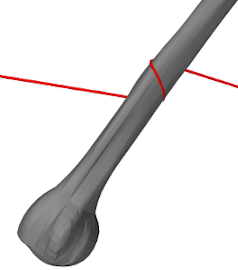
\includegraphics[]{images/HumerusWrap}&
 \includegraphics[]{images/HipWrap}
\else
 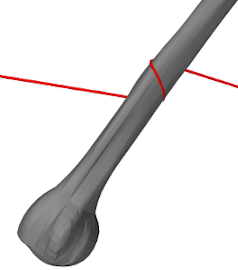
\includegraphics[width=2.5in]{images/HumerusWrap}&
 \includegraphics[width=2.5in]{images/HipWrap}
\fi
\end{tabular}
\end{center}
\caption{Muscle strands wrapped around general bone-shaped meshes: a
humerus (left), and a pelvis (right)}
\label{GeneralWrapping:fig}
\end{figure}

The second are general rigid bodies which are {\it not} analytic
subclasses, and for which the wrapping surface is determined directly
from the geometry of its collision mesh returned by
\javamethod[\mech.RigidBody]{getCollisionMesh()}.  (Typically the
collision mesh corresponds to the surface mesh, but it is possible to
specify alternates; see Section \ref{rigidBodyMultipleMeshes:sec}.)
This is useful in that it permits wrapping around {\it arbitrary} mesh
geometries (Figure \ref{GeneralWrapping:fig}), but in order for the
wrapping to work well, these geometries should be smooth, without
sharp edges or corners.  Wrapping around general meshes is implemented
using a quadratically interpolated signed-distance grid (Section
\ref{DistanceGrids:sec}), and the resolution of this grid also affects
the effective smoothness of the wrapping surface. More details on this
are given in Section \ref{GeneralSurfaceWrapping:sec}.

\subsection{Example: wrapping around a cylinder}
\label{CylinderWrapping:sec}

\begin{figure}[t]
\begin{center}
\iflatexml
 \includegraphics[]{images/CylinderWrappingStart}
\else
 \includegraphics[width=3.75in]{images/CylinderWrappingStart}
\fi
\end{center}
\caption{CylinderWrapping model loaded into ArtiSynth.}
\label{CylinderWrapping:fig}
\end{figure}

A example showing multipoint spring wrapping is given by {\tt
artisynth.demos.tutorial.CylinderWrapping}.  It consists of a
{\tt MultiPointSpring} passing through a single via point, with both
segments on either side of the point made wrappable. Two analytic
wrappables are used: a fixed {\tt RigidCylinder}, and a moving {\tt
RigidEllipsoid} attached to the end of the spring. The code, excluding
include directives, is given below: 

\lstset{numbers=left} 
\iflatexml
%% Hack: latexml lstinputlisting doesn't handle firstline correctly
\lstset{firstnumber={-15}}
\lstinputlisting[firstline=1]{../../src/artisynth/demos/tutorial/CylinderWrapping.java}
\lstset{firstnumber={1}}
\else
\lstinputlisting[firstline=17]{../../src/artisynth/demos/tutorial/CylinderWrapping.java}
\fi
\lstset{numbers=none}

Lines 4-17 of the {\tt build()} method create a {\tt MechModel} with
two fixed particles {\tt via0} and {\tt p1} to be used as via and stop
points. Next, two analytic wrappables are created: a {\tt
RigidCylinder} and a {\tt RigidEllipsoid}, with the former fixed in
place and the latter connected to the start of the spring via the
marker {\tt p0} (lines 20-37). Collisions are enabled between these
two wrappables at line 40. The spring itself is created (lines 44-52),
using {\tt setSegmentWrappable()} to make the segments ({\tt p0}, {\tt
via0}) and ({\tt via0}, {\tt p1}) wrappable with 50 knots each, and
{\tt addWrappable()} to make it aware of the two wrappables.  Finally,
render properties at set (lines 55-58), and a control panel (Section
\ref{ControlPanels:sec}) is added that allows the spring's {\sf
drawKnots} and {\sf drawABPoints} properties to be interactively set.

To run this example in ArtiSynth, select {\sf All demos > tutorial >
CylinderWrapping} from the {\sf Models} menu. The model should load and
initially appear as in Figure \ref{CylinderWrapping:fig}.  Running the
model will cause the ellipsoid to fall and the spring to wrap around
the cylinder. Using the pull tool
(Section ``Pull Manipulation'' in the
\artisynthManual{uiguide}{ArtiSynth User Interface Guide})
on the ellipsoid can cause additional motions and make it also collide
with the spring. Selecting {\sf drawKnots} or {\sf drawABPoints} in
the control panel will cause the spring to render its knots and/or A/B
points.

\section{General Surfaces and Distance Grids}
\label{GeneralSurfaceWrapping:sec}

As mentioned in Section \ref{ObstacleWrapping:sec}, wrapping around
general mesh geometries is implemented using a quadratically
interpolated signed distance grid. By default, for a rigid body, this
grid is generated automatically from the body's collision mesh (as
returned by {\tt getCollisionMesh()}; see Section
\ref{CollisionMeshesAndCompounds:sec}).

Using a distance grid allows very efficient collision handling between
the body and the wrap segment knots. However, it also means that the
true wrapping surface is not actually the collision mesh itself, but
instead the zero-valued isosurface associated with quadratic grid
interpolation.  Well-behaved wrapping behavior requires that this
isosurface be smooth and free of sharp edges, so that knot motions
remain relatively smooth as they move across it. Quadratic
interpolation helps with this, which is the reason for employing
it. Otherwise, one should try to ensure that (a) the collision mesh
from which the grid is generated is itself smooth and free of sharp
edges, and (b) the grid has sufficient resolution to not introduce
discretization artifacts.

Muscle wrapping is often performed around structures such as bones,
for which the representing surface mesh is often insufficiently smooth
(especially if segmented from medical image data).  In some cases, the
distance grid's quadratic interpolation may provide sufficient
smoothing on its own; to determine this, one should examine the
quadratic isosurface as described below. In other cases, it may be
necessary to explicitly smooth the mesh itself, either externally or
within ArtiSynth using the \javaclass[\mgeo]{LaplacianSmoother} class,
which can apply iterations of either Laplacian or volume-preserving
Taubin smoothing, via the method
%
\begin{lstlisting}[]
  LaplacianSmoother.smooth (mesh, numi, lam, mu);
\end{lstlisting}
%
Here {\tt numi} is the number of iterations and {\tt tau} and {\tt mu}
are the Taubin parameters. Setting ${\tt lam} = 1$ and ${\tt mu} = 0$
results in traditional Laplacian smoothing. If this causes the mesh to
shrink more than desired, one can counter this by setting {\tt tau}
and {\tt mu} to values used for Taubin smoothing, as described in
\cite{taubin1995curve}.

\begin{sideblock}
If the mesh is large (i.e., has many vertices), then smoothing it may
take noticeable computational time. In such cases, it is generally best
to simply save and reuse the smoothed mesh.
\end{sideblock}

By default, if a rigid body contains only one polygonal mesh, then its
surface and collision meshes (returned by
\javamethod[\mech.RigidBody]{getSurfaceMesh()} and
\javamethod[\mech.RigidBody]{getCollisionMesh()}, respectively) are
the same.  However, if it is necessary to significantly smooth or
modify the collision mesh, for wrapping or other purposes, it may be
desirable to use different meshes for the surface and collision. This
can be done by making the surface mesh non-collidable and adding an
additional mesh that {\it is} collidable, as discussed in Section
\ref{rigidBodyMultipleMeshes:sec} as illustrated by the following code
fragment:
%
\begin{lstlisting}[]
  PolygonalMesh surfaceMesh;
  PolygonalMesh wrappingMesh;

  // ... initialize surface and wrapping meshes ...

  // create the body from the surface mesh
  RigidBody body = RigidBody.createFromMesh (
      "body", mesh, /*density=*/1000, /*scale=*/1.0);

  // set the surface mesh to be non-collidable, and add the wrapping mesh as
  // collidable but not having mass
  body.getSurfaceMeshComp().setIsCollidable (false);
  RigidMeshComp wcomp = body.addMesh (
      wrappingMesh, /*hasMass=*/false, /*collidable=*/true);
  RenderProps.setVisible (wcomp, false); // hide the wrapping mesh
\end{lstlisting}
%
Here, to ensure that the wrapping mesh does {\it not} to contribute to
the body's inertia, its {\sf hasMass} property is set to false.

Although it is possible to specify a collision mesh that is separate
from the surface mesh, there is currently no way to specify {\it separate}
collision meshes for wrapping and collision handling.  If this is
desired for some reason, then one alternative is to create a separate
body for wrapping purposes, and then attach it to the main body, as
described in Section \ref{AlternateWrappingSurfaces:sec}.

To verify that the distance grid's quadratic isosurface is
sufficiently smooth for wrapping purposes, it is useful to visualize
the both distance grid and its isosurface directly, and if necessary
adjust the resolution used to generate the grid. This can be
accomplished using the body's
\javaclass[artisynth.core.mechmodels]{DistanceGridComp}, which is a
subcomponent named {\tt distanceGrid} and which may be obtained using
the method
%
\begin{lstlisting}
   DistanceGridComp getDistanceGridComp()
\end{lstlisting}
%
A {\tt DistanceGridComp} exports a number of properties that can be
used to control the grid's visualization, resolution, and fit around
the collision mesh. These properties are described in detail in
Section \ref{DistanceGrids:sec}, and can be set either in code using
their set/get accessors, or interactively using custom control panels
or by selecting the grid component in the GUI and choosing {\sf Edit
properties ...} from the right-click context menu.

\begin{sideblock}
When rendering the mesh isosurface, it is usually desirable to also
disable rendering of the collision meshes within the rigid body.  For
convenience, this can be accomplished by setting the body's {\sf
gridSurfaceRendering} property to {\tt true}, which will cause the
grid isosurface to be rendered {\it instead} of the body's meshes.
The isosurface type will be that indicated by the grid component's
{\sf surfaceType} property (which should be {\tt QUADRATIC} for the
quadratic isosurface), and the rendering will occur independently of
the visibility settings for the meshes or the grid component.
\end{sideblock}

\subsection{Example: wrapping around a bone}
\label{TalusWrapping:sec}

\begin{figure}[t]
\begin{center}
\begin{tabular}{cc}
\iflatexml
 \includegraphics[]{images/TalusWrapping}&
 \includegraphics[]{images/TalusWrapping2}
\else
 \includegraphics[width=3.2in]{images/TalusWrapping}&
 \includegraphics[width=3.2in]{images/TalusWrapping2}
\fi
\end{tabular}
\end{center}
\caption{TalusWrapping model, with a dragger being used to move {\tt
p0} (left), and the knots visible and grid visible with restricted
range (right).}
\label{TalusWrapping:fig}
\end{figure}

An example of wrapping around a general mesh is given by
{\tt artisynth.demos.tutorial.TalusWrapping}.  It consists
of a MultiPointSpring anchored by two via points and wrapped around a
rigid body representing a talus bone. The code, with include
directives omitted, is given below: 
\lstset{numbers=left}
\iflatexml
%% Hack: latexml lstinputlisting doesn't handle firstline correctly
\lstset{firstnumber={-12}}
\lstinputlisting[firstline=1]{../../src/artisynth/demos/tutorial/TalusWrapping.java}
\lstset{firstnumber={1}}
\else
\lstinputlisting[firstline=14]{../../src/artisynth/demos/tutorial/TalusWrapping.java}
\fi
\lstset{numbers=none}

The mesh describing the talus bone is loaded from the file {\tt
"data/TalusBone.obj"} located beneath the model's source directory
(lines 11-19), with the utility class
\javaclass[maspack.util]{PathFinder} used to determine the file path
(Section \ref{PathFinder:sec}).
To ensure better wrapping behavior, the mesh is smoothed
using Laplacian smoothing (line 21) before being used to create
the rigid body (lines 23-27). The spring and its anchor points {\tt
p0} and {\tt p1} are created between lines 30-49, with the talus added
as a wrappable. The spring contains a single segment which is made
wrappable using 100 knots, and initialized with an intermediate point
(line 45) to ensure that it wraps around the bone in the correct way.
Intermediate points are described in more detail in Section
\ref{wrappingInit:sec}.

Render properties are set at lines 52-56; this includes turning off
rendering for grid normals by zeroing the {\sf lineWidth} render
property for the grid component.

Finally, lines 59-67 create a control panel (Section
\ref{ControlPanels:sec}) for interactively controlling a variety of
properties, including {\sf gridSurfaceRendering} for the talus (to see
the grid isosurface instead of the bone mesh), {\sf resolution}, {\sf
maxResolution}, {\sf renderGrid}, and {\sf renderRanges} for the grid
component (to control its resolution and visibility), and {\sf
drawKnots} and {\sf wrapDamping} for the spring (to make knots visible
and to adjust the wrap damping as described in Section
\ref{wrapTuning:sec}).

To run this example in ArtiSynth, select {\sf All demos > tutorial >
TalusWrapping} from the {\sf Models} menu. Since all of the dynamic
components are fixed, running the model will not cause any initial
motion. However, while simulating, one can use the viewer's graphical
dragger fixtures (see the section ``Transformer Tools'' in the
\artisynthManual{uiguide}{ArtiSynth User Interface Guide}) to move
{\tt p0} or {\tt p1} and hence pull the spring across the bone surface
(Figure \ref{TalusWrapping:fig}, left). One can also interactively
adjust the property settings in the control panel to view the grid,
isosurface, and knots, and the adjust the grid's resolution.  Figure
\ref{TalusWrapping:fig}, right, shows the model with {\sf renderGrid}
and {\sf drawKnots} set to {\tt true} and {\sf renderRanges} set to
{\tt "10:12 * *"}.

\section{Initializing the Wrap Path}
\label{wrappingInit:sec}

By default, when a multipoint spring or muscle is initialized (either
at the start of the simulation or as a result of calling
\javamethod*[\mech .MultiPointSpring]{updateWrapSegments()}), each
wrappable segment is initialized to a straight line between its via
points. This path is then adjusted to avoid and wrap around obstacles,
using artificial linear forces as described in Section
\ref{wrapTuning:sec}. The result is a local shortest path that wraps
around obstacles instead of penetrating them.  However, in some cases,
the initial path may not be the one desired; instead, one may want it
to wrap around obstacles some other way. This can be achieved by
specifying additional intermediate points to initialize the segment as
a piecewise linear path which threads its way around obstacles in the
desired manner (Figure \ref{wrapInitialization:fig}).  These are
specified using the optional {\tt initialPnts} argument to the {\tt
setSegmentWrappable()} methods.

\begin{figure}[ht]
\begin{center}
 \includegraphics[width=6in]{images/wrapInitialization}
\end{center}
\caption{By default, the path for each wrappable segment is
initialized to a straight line between its via points (dotted line,
left), which is then adjusted to wrap around obstacles (solid line,
middle). To cause the path to wrap around obstacles in a different
way, it can instead be initialized using a piecewise-linear
path defined by intermediate initial points (dotted line, right),
which will then adjust to an alternate configuration.}
\label{wrapInitialization:fig}
\end{figure}

\begin{sideblock}
When initial points are specified, it is recommended to finish
construction of the spring or muscle with a call to
\javamethod[\mech.MultiPointSpring]{updateWrapSegments()}.  This fits
the wrappable segments to their correct path around the obstacles,
which can then be seen immediately when the model is first loaded. On
the other hand, by {\it omitting} an initial call to {\tt
updateWrapSegments()}, it is possible to see the initial path as
specified by the initial points. This may be useful to
verify that they are in the correct locations.
\end{sideblock}

\begin{sideblock}
In some cases, initial points may also be necessary to help ensure
that the initial path does not penetrate obstacles. While obstacle
penetration will normally be resolved by the artificial forces
described in Section \ref{wrapTuning:sec}, this may not always work
correctly if the starting path penetrates an obstacle too deeply.
\end{sideblock}

\subsection{Example: wrapping around a torus}
\label{TorusWrapping:sec}

\begin{figure}[ht]
\begin{center}
\iflatexml
 \includegraphics[]{images/TorusWrapping}
\else
 \includegraphics[width=3.75in]{images/TorusWrapping}
\fi
\end{center}
\caption{{\tt TorusWrapping} model loaded into ArtiSynth.}
\label{TorusWrapping:fig}
\end{figure}

An example of using initial points is given by {\tt
artisynth.demos.tutorial.TorusWrapping}, in which a spring
is wrapped completely around the inner section of a torus.
The primary code for
the build method is given below: 
\lstset{numbers=left}
\iflatexml
%% Hack: latexml lstinputlisting doesn't handle firstline correctly
\lstset{firstnumber={-20}}
\lstinputlisting[firstline=1,lastline=41]{../../src/artisynth/demos/tutorial/TorusWrapping.java}
\lstset{firstnumber={1}}
\else
\lstinputlisting[firstline=22,lastline=62]{../../src/artisynth/demos/tutorial/TorusWrapping.java}
\fi
\lstset{numbers=none}

The mech model is created in the usual way with frame and rotary
damping set to 1 and 10 (lines 4-5). The torus is created using the
analytic wrappable \javaclass[\mech]{RigidTorus} (lines 8-14). The
spring start and end points {\tt p0} and {\tt p1} are created at lines
(17-22), and the spring itself is created at lines (26-41), with six
initial points being specified to {\tt setSegmentWrappable()} to wrap
the spring completely around the torus inner section.

To run this example in ArtiSynth, select {\sf All demos > tutorial >
TorusWrapping} from the {\sf Models} menu. The torus will slide along
the wrapped spring until it reaches equilibrium.

\section{Alternate Wrapping Surfaces}
\label{AlternateWrappingSurfaces:sec}

Although it common to use the general mesh geometry of a {\tt
RigidBody} as the wrapping surface, situations may arise where it is
desirable to {\it not} do this. These may include:

\begin{itemize}

\item The general mesh geometry is not sufficiently smooth
to form a good wrapping surface;

\item Wrapping around the default mesh geometry is not stable, in
that it is too easy for the wrap strand to ``slip off'';

\item Using one of the simpler analytic geometries
(Table \ref{analyticWrappables:tbl}) may result in a more efficient
computation.

\end{itemize}

There are a couple of ways to handle this. One, discussed in Section
\ref{GeneralSurfaceWrapping:sec}, involves creating a collision mesh
which is separate from the general mesh geometry. However, that same
collision mesh must then also be used for collision handling (Chapter
\ref{ContactAndCollision:sec}). If that is undesirable, or if {\it
multiple} wrapping surfaces are needed, then a different approach may
be used. This involves creating the desired wrappable as a separate
object and then {\it attaching} it to the main {\tt
RigidBody}. Typically, this wrappable will be created with zero mass
(or density), so that it does not alter the effective mass or inertia
of the main body. The general procedure then becomes:

\begin{enumerate}

\item Create the main {\tt RigidBody} with whatever desired geometry
and inertia is needed;

\item Create the additional wrappable object(s), usually
with zero density/mass;

\item Attach the wrappables to the main body using
one of the {\tt MechModel} {\tt attachFrame()} methods described in
Section \ref{sec:mech:frameattachments}.

\end{enumerate}

\subsection{Example: wrapping for a finger joint}
\label{PhalanxWrapping:sec}

\begin{figure}[t]
\begin{center}
\iflatexml
 \includegraphics[]{images/PhalanxWrapping}
\else
 \includegraphics[width=3.75in]{images/PhalanxWrapping}
\fi
\end{center}
\caption{PhalanxWrapping model loaded into ArtiSynth.}
\label{PhalanxWrapping:fig}
\end{figure}

An example using an alternate wrapping surface is given by {\tt
artisynth.demos.tutorial.PhalanxWrapping}, which shows a 
a muscle wrapping around a joint between two finger
bones. Because the bones themselves are fairly narrow, using them as
wrapping surfaces would likely lead to the muscle slipping
off. Instead, a \javaclass[\mech]{RigidCylinder} is used for the
wrapping and attached to one of the bones. The code, with include
directives excluded, is given below: \lstset{numbers=left} \iflatexml
%% Hack: latexml lstinputlisting doesn't handle firstline correctly
\lstset{firstnumber={-17}}
\lstinputlisting[firstline=1]{../../src/artisynth/demos/tutorial/PhalanxWrapping.java}
\lstset{firstnumber={1}}
\else
\lstinputlisting[firstline=19]{../../src/artisynth/demos/tutorial/PhalanxWrapping.java}
\fi
\lstset{numbers=none}

The method {\tt createBody()} (lines 6-14) creates a rigid body from a
geometry mesh stored in a file in the directory ``{\tt data}'' beneath
the source directory, using the utility class
\javaclass[maspack.util]{PathFinder} used to determine the file path
(Section \ref{PathFinder:sec}).

Within the {\tt build()} method, a {\tt MechModel} is created
containing two rigid bodies representing the bones, {\tt proximal} and
{\tt distal}, with {\tt proximal} fixed and {\tt distal} free to move
with a frame damping of 0.03 (lines 18-28). A cylindrical joint is
then added between the bones, along with markers describing the
muscle's origin and insertion points (lines 31-42).  A {\tt
RigidCylinder} is created to act as a wrapping obstacle and attached
to the {\tt distal} bone in the same location as the joint (lines
46-50); since it is created with a density of 0 it has no mass and
hence does not affect the bone's inertia. The muscle itself is created
at lines 53-64, using a
\javaclass[artisynth.core.materials]{SimpleAxialMuscle} as a material
and an extra initial point specified to
{\tt setSegmentWrappable()} to ensure that it wraps around
the cylinder in the correct way (Section
\ref{wrappingInit:sec}). Finally, some render properties are set at lines
67-69.

To run this example in ArtiSynth, select {\sf All demos > tutorial >
PhalanxWrapping} from the {\sf Models} menu. The model should load and
initially appear as in Figure \ref{PhalanxWrapping:fig}.  When running
the model, one can move the {\tt distal} bone either
by using the pull tool (Section ``Pull
Manipulation'' in the
\artisynthManual{uiguide}{ArtiSynth User Interface Guide}),
or selecting the muscle in the GUI, invoking a property dialog by
choosing {\sf Edit properties ...} from the right-click context menu,
and adjusting the {\sf excitation} property.

\section{Tuning the Wrapping Behavior}
\label{wrapTuning:sec}

Wrappable segments are implemented internally using artificial linear
elastic forces to draw the knots together and keep them from
penetrating obstacles. These artificial forces are invisible to the
simulation: the wrapping segment has no mass, and the knot forces are
used to create what is essentially a first order physics that ``shrink
wraps'' each segment around the obstacles at the beginning of each
simulation step, forming a shortest-distance geodesic curve from
which the wrapping contact points A and B are calculated. This process
is now described in more detail.

Assume that a wrappable segment has $m$ knots, indexed by $k =
1, \ldots, m$, each located at a position $\x_k$. Two types of
artificial forces then act on each knot: a {\it wrapping force}
that pulls it closer to other knots, and {\it contact forces} that
push it away from wrappable obstacles. The wrapping force is given by
%
\begin{equation*}
\f_{w,k} = K_w (\x_{k+1} - 2 \x_k + \x_{k-1})
%\label{knotForce:eqn}
\end{equation*}
%
where $K_w$ is the {\it wrapping stiffness}. To determine the contact
forces, we compute, for each wrappable, the knot's distance to the
surface $d_k$ and associated normal direction $\n_k$, where $d_k < 0$
implies that the knot is inside. These quantities are determined
either analytically (for analytic wrappables, Table
\ref{analyticWrappables:tbl}), or using a signed distance grid (for
general wrappables, Section \ref{GeneralSurfaceWrapping:sec}).  The
contact forces are then given by
%
\begin{equation*}
\f_{c,k} = 
\begin{cases}
-K_c \, d_k \, \n_k & \text{if} \; d_k < 0 \\
0 & \text{otherwise},
\end{cases}
\end{equation*}
%
where $K_c$ is the {\it contact stiffness}.

The total force $\f_k$ acting on each knot is then given by
%
\begin{equation*}
\f_k = \f_{w,k} + \sum_c \f_{c,k}
%\label{XXX:eqn}
\end{equation*}
%
where the latter term is the sum of contact forces for all wrappables.
If we let $\x$ and $\f$ denote the aggregate position and force vectors
for all knots, then computing the wrap path involves finding the
equilibrium position such that $\f(\x) = 0$. This is done at the
beginning of each simulation step, or whenever \javamethod*[\mech
.MultiPointSpring]{updateWrapSegments()} is called, and
is achieved iteratively using Newton's method.
If $\x^j$ and $\f(\x^j)$ denote the positions and forces at iteration $j$, 
and
%
\begin{equation*}
\K \equiv \frac{\partial \f}{\partial \x}
\end{equation*}
%
denotes the local force derivative (or ``stiffness''), then the basic
Newton update is given by
%
\begin{equation*}
\x^{j+1} = \x^j - \K^{-1} \f(\x^j).
\label{NewtonSolve:eqn}
\end{equation*}
%
In practice, to help deal with the nonlinearities associated with
contact, we use a damped Newton update,
%
\begin{equation}
\x^{j+1} = \x^j + \alpha (D \I - \K)^{-1} \f(\x^j),
\label{DampedNewtonSolve:eqn}
\end{equation}
%
where $D$ is a constant {\it wrap damping} parameter, and $\alpha$ is
an adaptively computed step size adjustment. The computation of
(\ref{DampedNewtonSolve:eqn}) can be performed quickly, in $O(m)$
time, since $\K$ is a block-tridiagonal matrix, and the number of
iterations required is typically small (on the order of 10 or less),
particularly since the iterative procedure continues across simulation
steps and so $\f(\x)$ does not need to be brought to $0$ for any given
step. The maximum number of Newton iterations used for each
time step is $N_\text{max}$.

\begin{sideblock}
Again, it is important to understand the artificial knot forces
$\f(\x)$ described here are separate from the physical spring/muscle
tension forces $f(l,\dot l, a)$ discussed in Sections
\ref{AxialSprings:sec} and \ref{sec:mechii:musclematerials}, and {\it
only} facilitate the computation of each wrappable segment's path
around obstacles.
\end{sideblock}

The default values for the wrapping parameters are $K_w = 1$, $K_c =
10$, $D = 10$, and $N_\text{max} = 10$, and these often give
satisfactory results without the need for modification.  However, in
some situations the default muscle wrapping may not perform adequately
and it is necessary to adjust these parameters. Problems may include:

\begin{itemize}

\item The wrapping path does not settle down and tends to ``jump
around''.  Solutions include increasing the damping parameter $D$ or
the maximum number of wrap iterations $N_i$. For general wrapping
surfaces (Section \ref{GeneralSurfaceWrapping:sec}), one should also
ensure that the surface is sufficiently smooth.

\item A wrapping surface is too thin and so the wrapping
path ``jumps through'' it. Solutions include increasing the damping
parameter $D$, increasing the number of knots in the segment, or
decreasing the simulation step size. An alternative approach is to use
an alternative wrapping surface
(Section \ref{AlternateWrappingSurfaces:sec}) that is thicker and
better behaved.

\end{itemize}

Wrapping parameters are exported as properties of {\tt
MultiPointSpring} and {\tt MultiPointMuscle}, and may be changed in
code (using their set/get accessors), or interactively,
either by exposing them through a control panel,
or by selecting the spring/muscle in the GUI and choosing {\sf Edit
properties ...} from the right-click context menu.  Property values
include:

\begin{description}

\item[wrapStiffness] Wrapping stiffness $K_w$ between knot points
(default value 1). Since the wrapping behavior is determined by the
damping to stiffness {\it ratio}, it is generally not necessary to
change this value.

\item[wrapDamping] Damping factor $D$ (default
value 10). Increasing this value relative to $K_w$ results in wrap
path motions that are smoother and less likely to penetrate obstacles,
but which are also less dynamically responsive. Applications generally
work with damping values between 10 and 100 (assuming $K_w = 1$).

\item[contactStiffness] Contact stiffness $K_c$ used to resolve obstacle
penetration (default value 10). It is generally not necessary
to change this value. Decreasing it will increase the distance that
knots are permitted to penetrate obstacles, which {\it may} result in
a slightly more stable contact behavior.

\item[maxWrapIterations] Maximum number of Newton iterations
$N_\text{max}$ per time step (default value 10). If the wrapping
simulation exhibits instability, particularly with regard to obstacle
contact, increasing the number of iterations (to say 100) may help.

\end{description}

In addition, {\tt MultiPointSpring} and {\tt MultiPointMuscle} also
export the following properties to control the rendering of knot and
A/B points:

\begin{description}

\item[drawKnots] If true, renders the knot points in each wrappable segment.
This can be useful to visualize the knot density. Knots are rendered
using the style, size, and color given by the {\sf pointStyle},
{\sf pointRadius}, {\sf pointSize}, and {\sf pointColor} values of the
spring/muscle's render properties.

\item[drawABPoints] If true, renders the A/B points. These
are the first and last points of contact that a wrap segment makes
with each wrappable, and correspond to the
points where the spring/muscle's tension acts on that wrappable
(Section \ref{multipointSpringIntro:sec} and
Figure \ref{multiPointObstacle:fig}).  A/B points are rendered using
the style and size given by the {\sf pointStyle}, {\sf pointRadius}
($\times 1.2$) and {\sf pointSize} values of the spring/muscle's render
properties, and the color given by the {\sf ABPointColor} property.

\end{description}

\ifdefined\maindoc
\else
\end{document}
\fi
